% \input{\pSections "sec Nuclear Models"}
\section{Nuclear Models}

%\begin{frame}\frametitle{Popular Models of the Nucleus}
%\begin{enumerate}
%	\item \bl{Liquid Drop Model}
%	\item Shell Model
%	\item Quark Model
%\end{enumerate}
%\end{frame}

%%%   %%%   %%%   %%%
\subsection{Mysterious Nuclear Force}
\begin{frame}\frametitle{Strange Behavior of the Nuclear Force}
\center
	\href{\bethe}{
	\begin{overpic}[ scale = 0.65 ]
		{\pLocalGraphics /sa/bethe-title-a}
		\put(58,-3.5) {\includegraphics[ width = 1cm ]{\pLocalGraphics medal}}
	\end{overpic}}
	\ \\ \ \\
\footnotesize{\bl{Scientific American}, Vol. 189, No. 3 (September \bl{1953}), pp. 58-63}
\end{frame}

\begin{frame}\frametitle{Strange Behavior of the Nuclear Force}
\center
	\href{\bethe}{
	\begin{overpic}[ scale = 0.715 ]
		{\pLocalGraphics /sa/bethe-nuclear-force-a}
	\end{overpic}}
	\ \\ \ \\
\footnotesize{\bl{Scientific American}, Vol. 200, No. 1 (January \bl{1959}), pp. 75-84}
\end{frame}

\begin{frame}\frametitle{The Binding Force of Nucleons}
\center
	\href{\peierls}{
	\begin{overpic}[ scale = 0.8 ]
	% https://www.jstor.org/stable/10.2307/24944889
	{\pLocalGraphics /sa/sa-nucleus-a}
		%\put(-7,-10){Compute the temperature of the bar as a function of position.}
	\end{overpic}}
	\ \\ \ \\
\footnotesize{\bl{Scientific American}, Vol. 200, No. 1 (January \bl{1959}), pp. 75-84}
\end{frame}

\begin{frame}\frametitle{Vagaries of the Nuclear Force}
\center
	\href{\peierls}{
	\begin{overpic}[ scale = 0.15 ]
	{\pLocalGraphics /sa/nuclear-force}
	\end{overpic}}
	\ \\ \ \\[5pt]
		%
	\href{\peierls}{
	\begin{overpic}[ scale = 0.15 ]
	{\pLocalGraphics /sa/exchange}
	\end{overpic}}
\end{frame}

\begin{frame}\frametitle{Spin--Orbit Interactions}
\center
	\href{\peierls}{
	\begin{overpic}[ scale = 0.15 ]
	{\pLocalGraphics /sa/spin-orbit.jpg}
	\end{overpic}}
\end{frame}

\begin{frame}\frametitle{Popular Models of the Nucleus\jumpLittle}
\begin{enumerate}
	\item Liquid Drop Model: \bl{Fission}
	\item Shell Model: \bl{Energy Levels}
	\item Optical Model: Neutron capture \bl{cross section}
\end{enumerate}
\onedot
\end{frame}


%%%   %%%   %%%   %%%
\subsection{Optical Model}
\begin{frame}\frametitle{Popularization of the Optical Model}
\center
	\href{\weiskopf}{
	\begin{overpic}[ scale = 0.75 ]
	{\pLocalGraphics /sa/Weiskopf-a}
		%\put(-7,-10){Compute the temperature of the bar as a function of position.}
	\end{overpic}}
	\ \\ \ \\
\footnotesize{\bl{Scientific American}, Vol. 193, No. 6 (December \bl{1955}), pp. 84-91}
\end{frame}

\begin{frame}\frametitle{Cloudy Crystal Ball}
\center
	\href{\peierls}{
	\begin{overpic}[ scale = 0.2 ]
	{\pLocalGraphics /sa/cloudy}
		%\put(-7,-10){Compute the temperature of the bar as a function of position.}
	\end{overpic}}
\end{frame}

\begin{frame}\frametitle{Neutron Cross Section}
\center
	\href{\weiskopf}{
	\begin{overpic}[ scale = 0.090 ]
	{\pLocalGraphics /sa/crystal-ball}
		\put(85,64){\bl{theory}}
		\put(85,22){\bl{experiment}}
	\end{overpic}}
	\ \\ \ \\
\end{frame}

\begin{frame}\frametitle{Neutron Absorption}
\begin{table}[htp]
%\caption{default}
\begin{center}
\begin{tabular}{cc}
	\raisebox{2cm}{
	\href{\weiskopf}{
	\begin{overpic}[ scale = 0.65 ]
		{\pLocalGraphics /sa/na-text}
	\end{overpic}}} &
%
	\href{\weiskopf}{
	\begin{overpic}[ scale = 0.375 ]
		{\pLocalGraphics /sa/na-figures}
	\end{overpic}}
\end{tabular}
\end{center}
%\label{default}
\end{table}
\end{frame}

\begin{frame}\frametitle{Resonance}
\begin{table}[htp]
%\caption{default}
\begin{center}
\begin{tabular}{cc}
	\raisebox{3cm}{
	\begin{overpic}[ scale = 0.775 ]
		{\pLocalGraphics /sa/standing-wave-text}
	\end{overpic}} &
%
	\begin{overpic}[ scale = 0.355 ]
		{\pLocalGraphics /sa/standing-wave-figures}
	\end{overpic}
\end{tabular}
\end{center}
%\label{default}
\end{table}%
\onedot
\end{frame}

\begin{frame}\frametitle{Bonus Content: \href{https://en.wikipedia.org/wiki/Ramsauer\%E2\%80\%93Townsend\_effect}{Ramsauer-Townsend Effect}}
\center
	\href{https://aapt.scitation.org/doi/10.1119/1.1975094}{
	\begin{overpic}[ scale = 1.15 ]
	{\pLocalGraphics aapt-a}
		%\put(0,0){Text}
	\end{overpic}}
\end{frame}

\begin{frame}\frametitle{Bonus Content: \href{https://en.wikipedia.org/wiki/Ramsauer\%E2\%80\%93Townsend\_effect}{Ramsauer-Townsend Effect}}
\center
	\href{https://aapt.scitation.org/doi/10.1119/1.1975094}{
	\begin{overpic}[ scale = 1.15 ]
	{\pLocalGraphics aapt-a}
		\put(80,-10){\includegraphics[ width = 0.75in ]{\pLocalGraphics thyratron-04}}
	\end{overpic}}
\end{frame}

\begin{frame}\frametitle{Quantum Mechanical Scattering}
\center
	\href{https://physicsopenlab.org/2016/08/16/ramsauer-townsend-effect/}{
	\begin{overpic}[ scale = 0.15 ]
	{\pLocalGraphics potential-well}
		%\put(0,0){Text}
	\end{overpic}}
\end{frame}

\begin{frame}\frametitle{Quantum Mechanical Scattering\jumpLittle}
\center
	\href{https://physicsopenlab.org/2016/08/16/ramsauer-townsend-effect/}{
	\begin{overpic}[ scale = 0.65 ]
	{\pLocalGraphics potential-well-02}
		%\put(0,0){Text}
	\end{overpic}}
\end{frame}

%%%   %%%   %%%   %%%
\subsection{Shell Model}
\begin{frame}\frametitle{Borrow From Atomic Physics}
\center
	\href{\mayer}{
	\begin{overpic}[ scale = 0.65 ]
		{\pLocalGraphics /sa/mayer-a}
	\put(60,-3.5) {\includegraphics[ width = 1cm ]{\pLocalGraphics medal}}
	\end{overpic}}
	\ \\ \ \\
\footnotesize{\bl{Scientific American}, Vol. 184, No. 3 (March \bl{1951}), pp. 22-27}
\end{frame}

\begin{frame}\frametitle{Atomic Physics: Shell Names}
\center
	\href{https://en.wikipedia.org/wiki/Bohr_model}{
	\begin{overpic}[ scale = 0.35 ]
		{\pLocalGraphics wiki-bohr-atom}
		\footnotesize{
		\put(105,70){\rd{K} shell full at \bl{2}}
		\put(105,50){\rd{L} shell full at \bl{8}}
		\put(105,30){\rd{M} shell full at \bl{18}}}
	\end{overpic}}
\end{frame}

\begin{frame}\frametitle{Atomic Physics: Electron Shell, Subshell Names}
\center
	\href{https://en.wikipedia.org/wiki/Electron_shell}{
	\begin{overpic}[ scale = 0.16 ]
	{\pLocalGraphics wiki-electron-K}
	\end{overpic}}
\end{frame}

\begin{frame}\frametitle{Atomic Physics: Electron Shells}
\center
	\href{https://en.wikipedia.org/wiki/Electron_shell}{
	\begin{overpic}[ scale = 0.25 ]
	{\pLocalGraphics wiki-electron-orbits}
	\end{overpic}}
\end{frame}

\begin{frame}\frametitle{Atomic Physics: Electron Shells}
\center
	\href{https://en.wikipedia.org/wiki/Electron_shell}{
	\begin{overpic}[ scale = 0.25 ]
	{\pLocalGraphics wiki-electron-s}
	\end{overpic}}
\end{frame}

\begin{frame}\frametitle{Atomic Physics: Filling the Shells}
\center
	\href{https://en.wikipedia.org/wiki/Electron_shell}{
	\begin{overpic}[ scale = 0.45 ]
	{\pLocalGraphics wiki-electron-arrows}
	\end{overpic}}
\end{frame}

\begin{frame}\frametitle{Shell Levels}
\center
	\href{\peierls}{
	\begin{overpic}[ scale = 0.175 ]
	{\pLocalGraphics /sa/shells}
	\end{overpic}}
\end{frame}

\begin{frame}\frametitle{Shell Theory Magic Numbers}
\center
	\href{\mayer}{
	\begin{overpic}[ scale = 0.175 ]
	{\pLocalGraphics /sa/nuclides}
	\end{overpic}}
\end{frame}

\begin{frame}\frametitle{Margenau: Naieve Shell Levels}
\center
	\href{\mayer}{
	\begin{overpic}[ scale = 0.55 ]
	{\pLocalGraphics /sa/mayer-margenau-a}
	\end{overpic}}
\end{frame}

\begin{frame}\frametitle{Spin--Orbit Interactions}
\center
	\href{\peierls}{
	\begin{overpic}[ scale = 0.15 ]
	{\pLocalGraphics /sa/spin-orbit.jpg}
	\end{overpic}}
\end{frame}

\begin{frame}\frametitle{Mayer: Corrected Shell Levels}
\center
	\href{\mayer}{
	\begin{overpic}[ scale = 0.55 ]
	{\pLocalGraphics /sa/mayer-mayer-a}
	\end{overpic}}
\end{frame}

\begin{frame}\frametitle{Wikipedia: Nuclear Shell Model}
\center
	\href{https://en.wikipedia.org/wiki/Nuclear_shell_model}{
	\begin{overpic}[ scale = 0.35 ]
	{\pLocalGraphics wiki-magic-numbers}
	\end{overpic}}
\end{frame}

\begin{frame}\frametitle{Wikipedia: Nuclear Shell Model\jumpLittle}
\center
	\href{https://en.wikipedia.org/wiki/Nuclear_shell_model}{
	\begin{overpic}[ scale = 0.275 ]
	{\pLocalGraphics wiki-shell-diagram}
	\end{overpic}}
	\twodots
\end{frame}

%%%   %%%   %%%   %%%
\subsection{Liquid Drop Model}
%
\begin{frame}\frametitle{Summary of Liquid Drop Model}
\begin{enumerate}
	\item Nucleus is liquid drop %$\Rightarrow \Longrightarrow$
	\item Fluid is incompressible
	\item Volume is conserved
\end{enumerate}
\end{frame}

\begin{frame}\frametitle{Fission of a Liquid Drop}
\center
	\href{http://www.jstor.org/stable/24950391}{
	\begin{overpic}[ scale = 0.25 ]
	{\pLocalGraphics fission-drops}
		%\put(0,0){Text}
	\end{overpic}}
\end{frame}

\begin{frame}\frametitle{Deformation of Spherical Drop}
\center
	\href{https://www.slideshare.net/cscottthomas/ch-32-radiation-nuclear-energy-and-particles-online}{
	\begin{overpic}[ scale = 0.225 ]
	{\pLocalGraphics fission/ld-fission}
		%\put(-7,-10){Compute the temperature of the bar as a function of position.}
	\end{overpic}}
\end{frame}
%
\begin{frame}\frametitle{Interactions Within the Liquid Drop}
\center
	\href{https://en.wikipedia.org/wiki/Semi-empirical_mass_formula}{
	\begin{overpic}[ scale = 0.2 ]
	{\pLocalGraphics wiki/liquid-drop-options}
		%\put(-7,-10){Auxiliary text.}
	\end{overpic}}
\end{frame}
%
%\begin{frame}\frametitle{Fission of a Liquid Drop}
%\center
%	\href{\fermiBook}{
%	\begin{overpic}[ scale = 0.1 ]
%	{\pLocalGraphics fermi/fermi-splash}
%		%\put(0,0){Text}
%	\end{overpic}}
%\end{frame}
%
%\begin{frame}\frametitle{Fission of a Liquid Drop}
%\center
%	\href{\fermiBook}{
%	\begin{overpic}[ scale = 1.0 ]
%	{\pLocalGraphics fermi/fermi-text-01-a}
%		%\put(0,0){Text}
%	\end{overpic}}
%\end{frame}

\begin{frame}\frametitle{Fission of a Liquid Drop}
\center
	\href{\fermiBook}{
	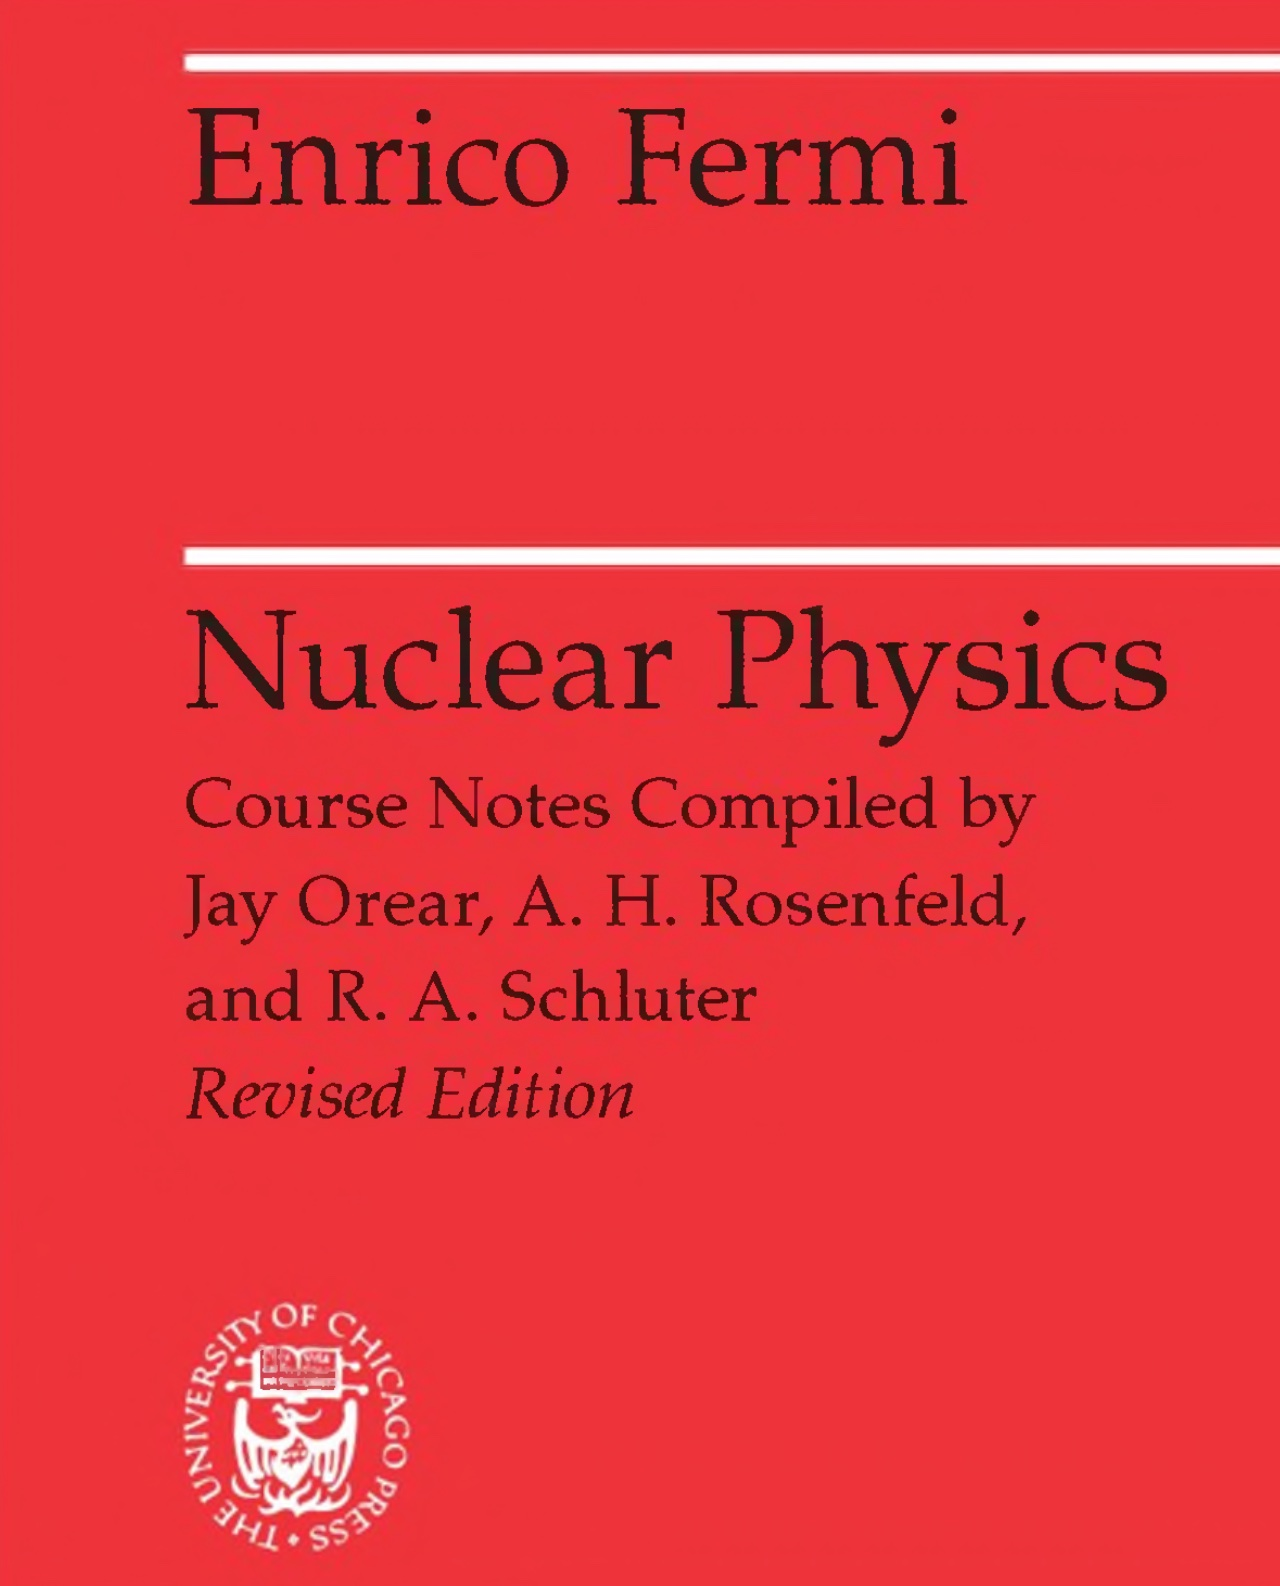
\includegraphics[ width = 1.25in ]{\pLocalGraphics fermi/fermi-splash}}
	\href{\fermiBook}{
	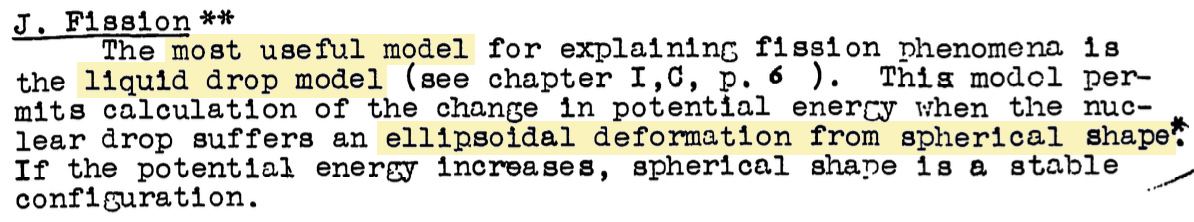
\includegraphics[ width = 4.5in ]{\pLocalGraphics fermi/fermi-text-01-a}}
\end{frame}

\begin{frame}\frametitle{Fission of a Liquid Drop\jumpLittle}
\center
	\href{\fermiBook}{
	\begin{overpic}[ scale = 0.175 ]
	{\pLocalGraphics fermi/fermi-text-02}
	\end{overpic}}
\end{frame}



%%%   %%%   %%%   %%%
\subsection{Fission Limit Using Liquid Drop}

\begin{frame}\frametitle{\href{https://en.wikipedia.org/wiki/Drop_(liquid)}{Water Drop}}

\begin{table}[htp]
%\caption{default}
\begin{center}
\begin{tabular}{cccc}
		%
	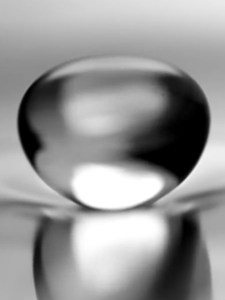
\includegraphics[ width = 1in ]{\pLocalGraphics animation/drop-0} & 
	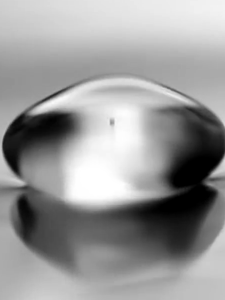
\includegraphics[ width = 1in ]{\pLocalGraphics animation/drop-20} & 
	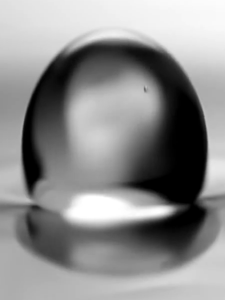
\includegraphics[ width = 1in ]{\pLocalGraphics animation/drop-40} & 
	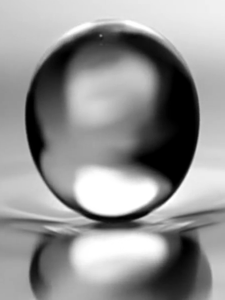
\includegraphics[ width = 1in ]{\pLocalGraphics animation/drop-60} 
		%
\end{tabular}
\end{center}
%\label{default}
\end{table}
\mg{\tiny{\texttt{By A7N8X - Own work, CC BY-SA 4.0, \href{https://commons.wikimedia.org/w/index.php?curid=48828510}{https://commons.wikimedia.org/w/index.php?curid=48828510}}}}
\end{frame}


\begin{frame}\frametitle{Comparison of Liquid Drop Models}
\begin{table}[htp]
%\caption{default}
\begin{center}
\begin{tabular}{cc}
	Constant Radius & Variable Radius \\\hline
	\ \\
	\includegraphics[ width= 2in ]{\pLocalGraphics serber} & 
	\includegraphics[ width= 2in ]{\pLocalGraphics bohr-wheeler} 
\end{tabular}
\end{center}
%\label{default}
\end{table}%
\end{frame}

\begin{frame}\frametitle{Two Schools of Thought\jumpBig}
\begin{table}[htp]
%\caption{default}
\begin{center}
\begin{tabular}{ccc}
	\bl{Constant} Radius && \pr{Variable} Radius \\\hline
	\ \\ 
	\serberPhoto && 
		\bohrPhoto \quad \wheelerPhoto\\
	\bl{\serber} && \multicolumn{1}{l}{\qquad \phantom{e} \pr{\bohr} \qquad \qquad \quad \pr{\wheeler}}
\end{tabular}
\end{center}
%\label{default}
\end{table}%
\end{frame}


\endinput  %  ==  ==  ==  ==  ==  ==  ==  ==  ==
